\RequirePackage{fix-cm}
\documentclass[11pt,a4paper,twoside]{vutinfth}

% useful packages
\usepackage{graphicx,
            textpos}
\usepackage{float}
\usepackage{helvet}
\usepackage{lipsum}
\usepackage{amsmath}
\usepackage{fancyhdr}
\usepackage{multicol}
\usepackage{setspace}
\usepackage[super, numbers]{natbib}
\usepackage{emptypage}
\usepackage[linktocpage=true]{hyperref}
\usepackage[toc,acronym,nonumberlist]{glossaries}
\usepackage{tocloft}
\usepackage{wrapfig}
\makeglossaries


% Import packages for drawing diagram
%More defined colors
\usepackage[dvipsnames]{xcolor}
% Required package
\usepackage{tikz}
\usetikzlibrary{positioning}

% Load packages to allow in- and output of non-ASCII characters.
\usepackage{lmodern}        % Use an extension of the original Computer Modern font to minimize the use of bitmapped letters.
\usepackage[T1]{fontenc}    % Determines font encoding of the output. Font packages have to be included before this line.
\usepackage[utf8]{inputenc} % Determines encoding of the input. All input files have to use UTF8 encoding.

% Extended LaTeX functionality is enables by including packages with \usepackage{...}.
\usepackage{amsmath}    % Extended typesetting of mathematical expression.
\usepackage{amssymb}    % Provides a multitude of mathematical symbols.
\usepackage{mathtools}  % Further extensions of mathematical typesetting.
\usepackage{microtype}  % Small-scale typographic enhancements.
\usepackage[inline]{enumitem} % User control over the layout of lists (itemize, enumerate, description).
\usepackage{multirow}   % Allows table elements to span several rows.
\usepackage{booktabs}   % Improves the typesettings of tables.
\usepackage{subcaption} % Allows the use of subfigures and enables their referencing.
\usepackage[ruled, lined, linesnumbered, commentsnumbered, longend]{algorithm2e} %
%Enables the writing of pseudo code.
%\usepackage[usenames,dvipsnames,table]{xcolor} % Allows the definition and use o colors.
%This package has to be included before tikz.
\usepackage{nag}       % Issues warnings when best practices in writing LaTeX documents are violated.
\usepackage{todonotes} % Provides tooltip-like todo notes.
\usepackage{hyperref}  % Enables cross linking in the electronic document version. This package has to be included second to last.
\usepackage[acronym,toc]{glossaries} % Enables the generation of glossaries and lists fo acronyms. This package has to be included last.

% Define convenience functions to use the author name and the thesis title in the PDF document properties.
\newcommand{\authorname}{Jan Stevens} % The author name without titles.
\newcommand{\thesistitle}{Coarse grained simulations of the DNA nanopistion} % The title

% Set PDF document properties
\hypersetup{
    pdfpagelayout   = TwoPageRight,           % How the document is shown in PDF viewers (optional).
    pdfauthor       = {\authorname},          % The author's name in the document
    pdftitle        = {\thesistitle},         % The document's title in the document
    pdfsubject      = {Master Thesis: Jan Stevens},              % The document's subject
    pdfkeywords     = {Thesis, Physics, DNA, Simulations}, % The document's keywords in
    colorlinks      = true,
    allcolors       = blue,
    linkbordercolor = {white}
}

\setpnumwidth{2.5em}        % Avoid overfull hboxes in the table of contents (see memoir

\setsecnumdepth{subsection} % Enumerate subsections.

\nonzeroparskip             % Create space between paragraphs (optional).
\setlength{\parindent}{0pt} % Remove paragraph identation (optional).

\makeindex      % Use an optional index.
\makeglossaries % Use an optional glossary.
\glstocfalse   % Remove the glossaries from the table of contents.


% settings for table of contents and section numbering
\setcounter{secnumdepth}{1} % numbering to which sublevel?
\setcounter{tocdepth}{1} % How many levels does the table of contents have?

\newcommand*\cleartoleftpage{%
  \clearpage
  \ifodd\value{page}\hbox{}\newpage\fi
}

% page settings
%\topmargin -10mm
%\textwidth 160truemm
%\textheight 240truemm
%\oddsidemargin 0mm
%\evensidemargin 0mm


% define the KUL colors
\definecolor{green}{RGB}{172,196,0}
\definecolor{bluetitle}{RGB}{29,141,176}
\definecolor{blueaff}{RGB}{0,0,128}
\definecolor{blueline}{RGB}{82,189,236}

% define units for the text blocks
\setlength{\TPHorizModule}{1mm}
\setlength{\TPVertModule}{1mm}

% Define your symbols and acronyms in here
% Used to give a list of symbols in Glossary on page vii
\newglossaryentry{pi}
{
  name={\ensuremath{\pi}},
  description={ratio of circumference of circle to its
               diameter},
  sort=pi
}

\newglossaryentry{alpha}
{
  name={\ensuremath{\alpha}},
  description={a random greek letter},
  sort=alpha
}

% Used to give a list of Acronyms in Acronyms on page ix
\newacronym{LSS}{LSS}{landslide susceptibility}


% Remove rule and put quote on the left of page
\renewcommand{\epigraphflush}{center}
%\renewcommand{\epigraphflush}{flushleft}

\epigraphfontsize{\small\itshape}
\setlength\epigraphwidth{9cm}
\setlength\epigraphrule{1pt}

\newenvironment{smallfont}{\fontfamily{lmodern}\small\selectfont}{\par}

% Start of the actual document
\begin{document}

\selectlanguage{english}

\newcommand\mycommfont[1]{\small\ttfamily\textcolor{blue}{#1}}
\SetCommentSty{mycommfont}

% FRONT MATTER
\frontmatter
\rmfamily

\thispagestyle{empty}
\newcommand{\form}[1]{\scalebox{1.087}{\boldmath{#1}}}
\sffamily
%
\begin{textblock}{191}(-17,-20)
    \colorbox{green}{\hspace{123mm}\
    \hspace{20mm}\parbox[c][18truemm]{48mm}{\textcolor{white}{FACULTY OF SCIENCES}}}
\end{textblock}
%
\begin{textblock}{70}(-11,-27)
\textblockcolour{}
\includegraphics*[height=19.8truemm]{Figures/LogoKULeuven}
\end{textblock}
%
\begin{textblock}{160}(-6,26)
\textblockcolour{}
\vspace{-\parskip}
\flushleft
\fontsize{40}{38}\selectfont \textcolor{bluetitle}{Coarse-grained simulations of the DNA
nanopiston}\\[1.5mm]
%\fontsize{20}{22}\selectfont subtitle \form{$S=\pi r^2$\textsl{(optional)}}
\end{textblock}
%
%\begin{textblock}{160}(8,147)
%\textblockcolour{}
%\vspace{-\parskip}
%\flushright
%\fontsize{14}{16}\selectfont \textbf{Jan Stevens}
%\end{textblock}
%
\begin{textblock}{160}(8,161)
\textblockcolour{}
\vspace{-\parskip}
\flushright
\fontsize{14}{16}\selectfont \textbf{Jan Stevens}
\end{textblock}
%
\begin{textblock}{70}(-6,185)
\textblockcolour{}
\vspace{-\parskip}
\flushleft
Supervisor: Prof. E. Carlon\\[-2pt]
\textcolor{blueaff}{Affiliation \textsl{(optional)}}\\[5pt]
Tutor: \textsl{(optional)}\\[-2pt]
\textcolor{blueaff}{Affiliation \textsl{(optional)}}\\
\end{textblock}
%
\begin{textblock}{160}(8,185)
\textblockcolour{}
\vspace{-\parskip}
\flushright
Thesis presented in\\[4.5pt]
fulfillment of the requirements\\[4.5pt]
for the degree of Master of Science\\[4.5pt]
in Physics
\end{textblock}
%
\begin{textblock}{160}(8,224)
\textblockcolour{}
\vspace{-\parskip}
\flushright
Academic year 2020-2021
\end{textblock}
%
\begin{textblock}{191}(-17,237)
{\color{blueline}\rule{550pt}{5.5pt}}
\end{textblock}
%
%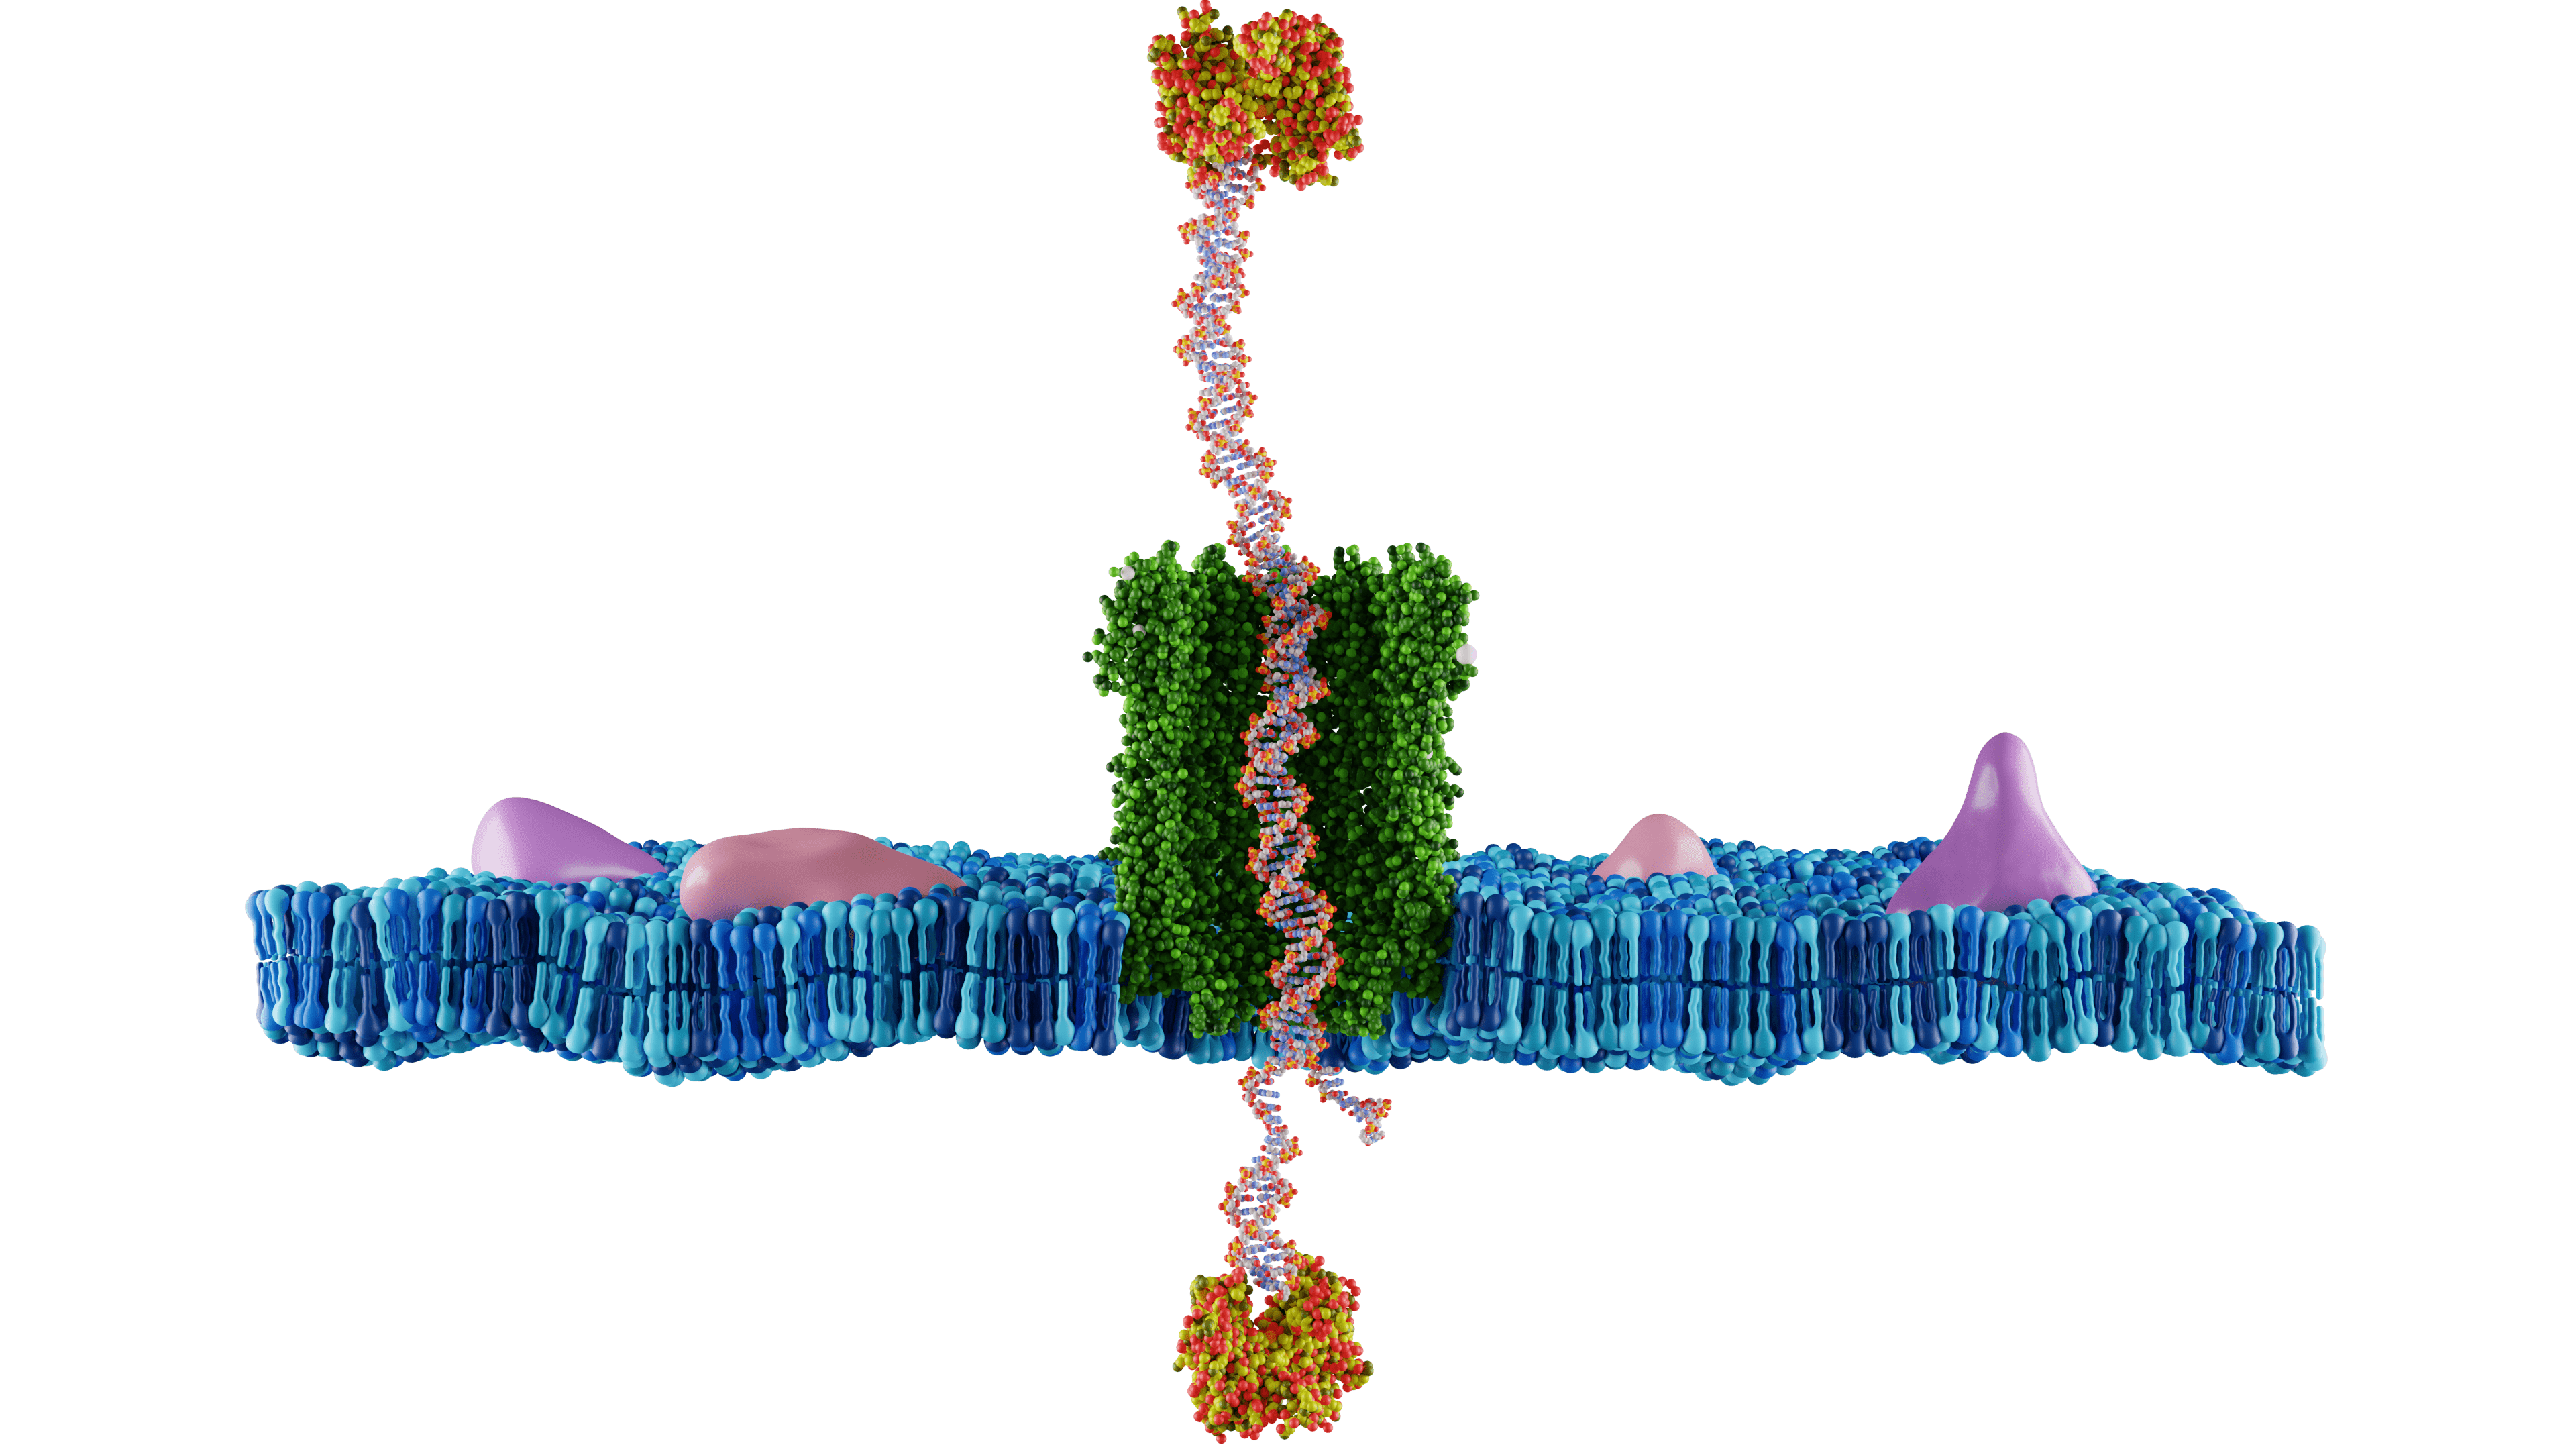
\includegraphics[height=9.5cm, width = 15.5cm]{Figures/CoverPhoto.png}
\vspace*{5.7cm}
\begin{center}
\begin{figure}[H]
\centering
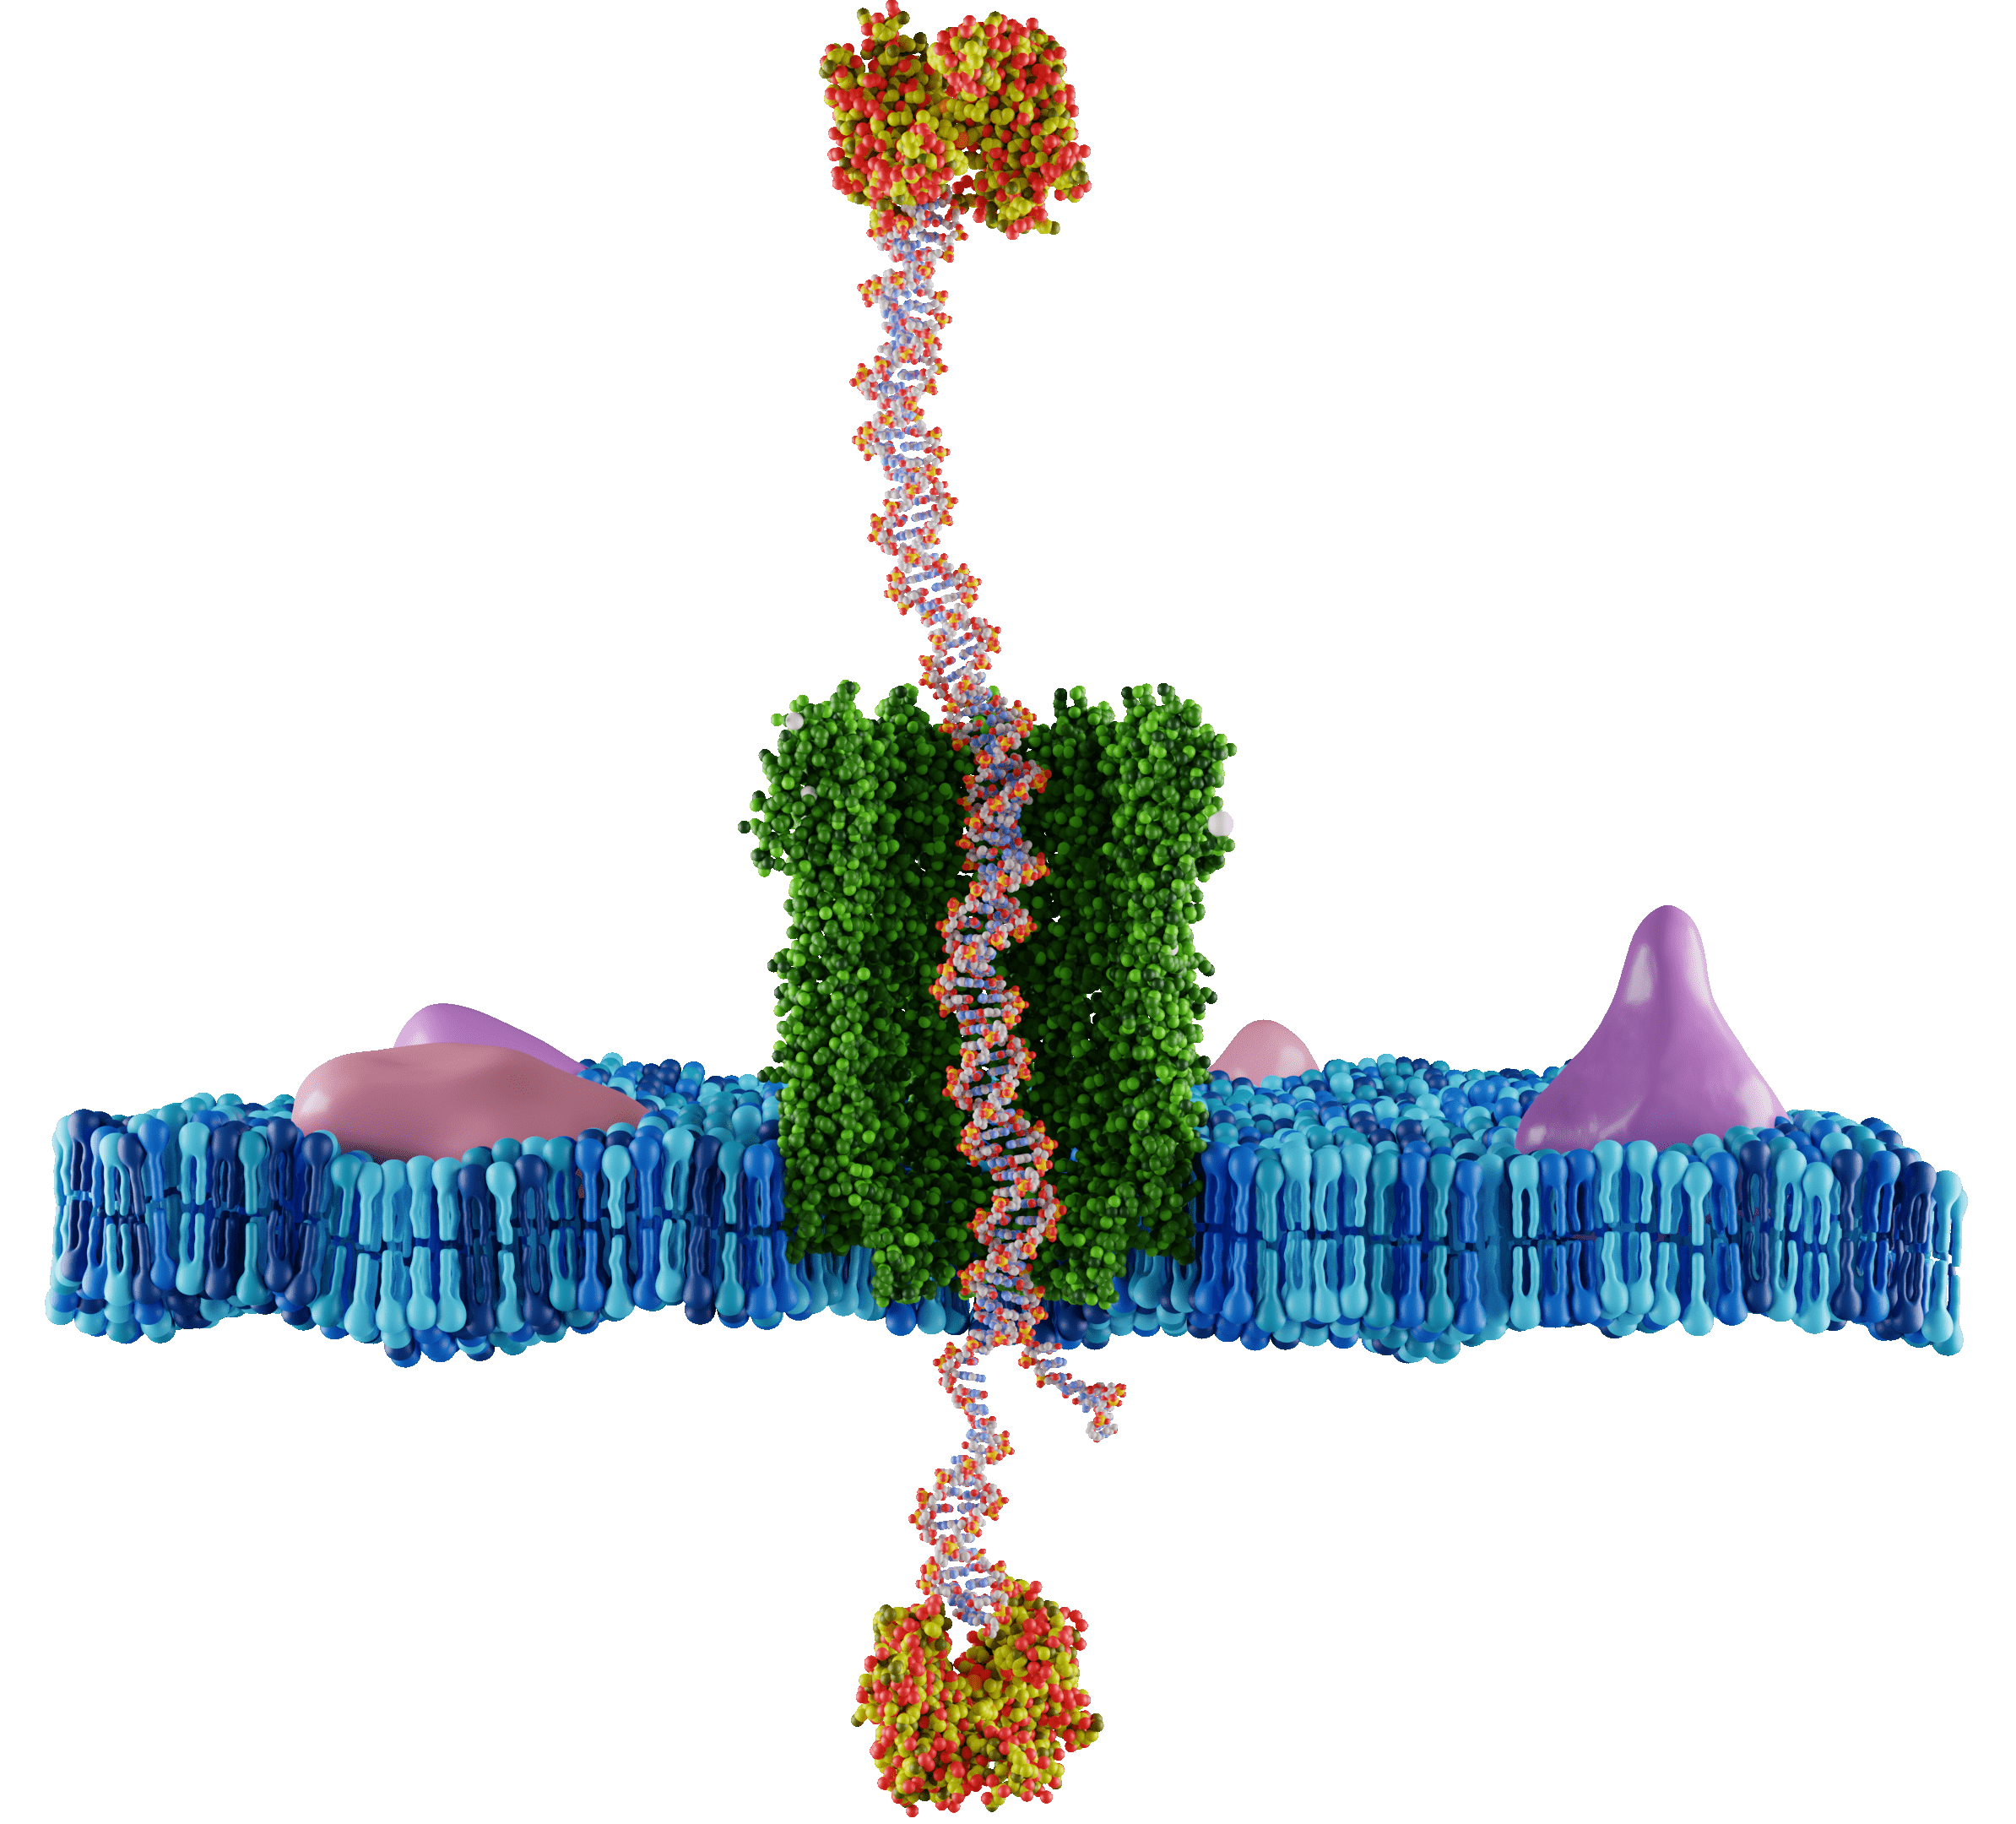
\includegraphics[scale=0.166]{Figures/CoverPhoto2.png}
\end{figure}
\end{center}
%
\vfill
 \cleardoublepage
\thispagestyle{empty}
\setlength{\parindent}{0cm}
\vspace*{\fill}

\begin{smallfont}
\copyright\ Copyright by KU Leuven \par
Without written permission of the promoters and the authors it is forbidden to reproduce or adapt in any form or by any means any part of this publication. Requests for obtaining the right to reproduce or utilize parts of this publication should be addressed to KU Leuven, Faculteit Wetenschappen, Geel Huis, Kasteelpark Arenberg 11 bus 2100, 3001 Leuven (Heverlee), Telephone +32 16 32 14 01.
A written permission of the promoter is also required to use the methods, products, schematics and programs described in this work for industrial or commercial use, and for submitting this publication in scientific contests.
\end{smallfont}

\setlength{\parindent}{0.5cm}
 \cleardoublepage
\setcounter{page}{0}
\pagenumbering{roman}

\addcontentsline{toc}{chapter}{Abstract}
\chapter*{Abstract}

Autonomous molecular machines are ubiquitous in the machinery of life, collectively
driving the molecular processes in our cells. Inspired by these biological machines,
scientists
develop synthetic devices performing specialised operations at the nanoscale. In this
thesis we study a specific molecular machine designed by Bayoumi et al.\cite{Bayoumi21},
which is composed of a DNA-neutravidin piston trapped inside a ClyA nanopore.

Using the free energy of DNA hybridisation this molecular machine is able to perform
autonomous and active transport of DNA cargo both following or opposing an
external bias force. During each operating cycle of the nanopiston a DNA cargo
is transported from the cis- to the trans-side of the membrane, in which the piston is
embedded.

Due to the length scale associated with molecular machines performing in depth
experimental studies has been proven to be challenging. During this thesis we aim
to shed light on the operating principles of the nanopiston by using molecular dynamics
simulations. Motivated by the computational cost of classical all-atom simulations a
coarse-grained model of the DNA nanopiston is designed.

Entropic interactions between the DNA piston and the nanopore are thought to
play an important role in facilitating the DNA transport. Studying these effects reveal
two distinct origins of entropic forces. Large double stranded DNA is kept predominantly
outside of the pore's constriction, by the entropic penalty of confinement.  Whereas, the
flexible single stranded DNA also
endouvours to maximize its available configurational space by opposing confinement.

Consecutively the  conformational fluctuations of
the nanopiston are studied.  These simulations clearly show the importance of the
entropic interactions promoting the operation cycle.  The entropic
penalty of confining the flexible single stranded DNA components of the piston in the
nanopore enable the continuation of the hybridisation reactions.

In an attempt to study a full piston cycle, the hybridisation reactions driving the
operation are simulated using our coarse-grained
model. Due to the inherent difficulty of simulating these reactions an advanced
sampling method called forward flux sampling is needed.
While performing these simulations the main limitation of our coarse-grained model is
encountered. The compliance of the biological nanopore is found to be essential in
facilitating the hybridisation pathways, but is not yet incorporated in our current
model.

\cleardoublepage
\cleardoublepage
\addcontentsline{toc}{chapter}{Samenvatting}
\chapter*{Samenvatting}
Summary in dutch.

\cleardoublepage
\addcontentsline{toc}{chapter}{Summary}
\chapter*{Summary}
Summary in english.
 \cleardoublepage
\printglossaries \cleardoublepage
%\addcontentsline{toc}{chapter}{List of Figures}
\listoffigures \cleardoublepage
%\addcontentsline{toc}{chapter}{List of Tables}
\listoftables \cleardoublepage
%\addcontentsline{toc}{chapter}{Contents}
\linespread{0.9}
{\small \tableofcontents}
\cleardoublepage
\linespread{1}

% MAIN MATTER
\mainmatter
\setcounter{page}{0}
\pagenumbering{arabic}

%% Introduction
\chapter{Introduction}
\vspace{-1cm}
\epigraphfontsize{\small\itshape}
\epigraph{“...if we were to name the most powerful assumption of all, which leads one on
and on in an attempt to understand life, it is that all things are made of atoms, and
that everything that living things do can be understood in terms of the jigglings and
wigglings of atoms.”}
{--- \textup{Richard P. Feynman}, The Feynman Lectures on Physics\cite{feynmanLectures}}
\section{Thesis outline}

All organisms in nature tirelessly perform work to keep their cellular functions
intact, opposing the ever increasing entropy in their environment. This work is
collectively performed by countless molecular machines, all contributing to
their specific tasks.

Despite being so abundantly present in nature, fabricating synthetic molecular machines
turns out to be a difficult task. One of the biggest hurdles in this process arises from
their corresponding length-scale. Often times these machines are not larger then
a few nanometres, making the typical energy associated with the bonds and
distortions of their structure comparable to thermal energy fluctuations. As a result of
these thermal fluctuations in their environment molecular machines naturally perform
a stochastic motion that complicates their functioning.  Extracting useful work from
these freely tumbling structures is almost impossible. To overcome this limitation most
synthetic molecular machines are embedded in a larger complex providing necessary
stability.\cite{Watson2016}

This phenomenon is also observed in nature, for instance in the interfacing of protein
complexes with the phospholipid bilayer of cells.  A wildly known example is the
bacterial flagellar motor, shown in Figure \ref{fig:flagella}. The function of this
machine is providing an efficient way for bacteria to
roll and tumble throughout their environment. Just like in electrical motors, the
flagellar motor consists of a stator and a rotor. The stator is anchored into the cell
membrane,
while the rotor is allowed to freely rotate. The work is produced by the flow of cations
through the stator. Inducing changes in the electrostatic interactions between the two
parts of the flagellar motor generates a unidirectional motion.\cite{sowa_berry_2008}

Similarly to macroscopic engines, heat is produced during the operation of molecular
machines. When the structure is not capable of dissipating this heat efficiently, an
excessive build-up compromises its durability. To mitigate this problem, large and soft
molecules are often used in the design of nanomachines. A logical choice
is the use of polymers, which can effectively dissipate heat as a result of their
flexibility.  Due to the programmability of DNA, using the Watson-Crick interactions,
the DNA polymer provides additional aptitude. This makes DNA a popular material in
nanotechnology.

The central topic of this thesis is studying a synthetic molecular machine consisting of
a DNA nanopiston embedded into a phospholipid membrane, as depicted on the cover page.
The structure was designed by Bayoumi et al. with the aim of performing
selective transport of DNA through a membrane.\cite{Bayoumi21} This
nanopiston can be characterised as an autonomous molecular machine, which turns over
chemical fuel to continuously perform work.

% The operation cycle of previously designed DNA transporters requires a supporting
% external bias.\cite{Franceschini2013} However, this specific nanopiston also operates
% opposing an external bias force. The physics driving this machine is entropy and will be
% discussed in detail in throughout this thesis.

In the first chapter a comprehensive introduction of important concepts
regarding the DNA nanopiston is given. Having laid this theoretical foundation, the
structure and operation cycle of the DNA nanopiston is discussed in chapter two. Next the
computational model used in this thesis is presented in chapter three. In chapter four,
the results of these simulations is discussed. Finally chapter five will offer a
discussion of these results and recommendations for further research.
\vspace{0.5cm}
\begin{figure}[ht!]
\begin{center}
  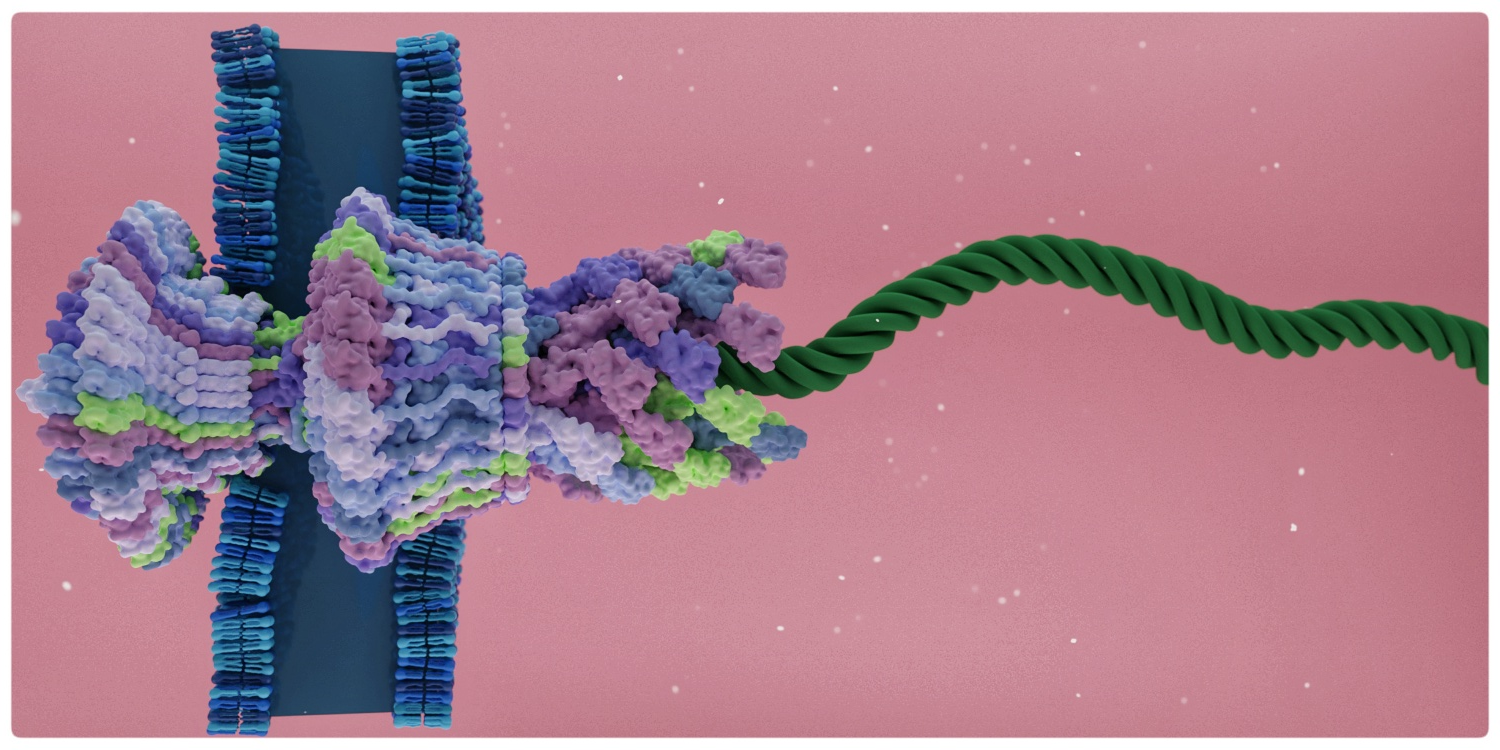
\includegraphics[width=0.85\textwidth]{Figures/flagella2.png}
  \caption[Render of a flagellar motor-hook complex, based on the cryo-EM structure of
  the Salmonella flagellar motor.] {Render of a flagellar motor-hook complex embedded in
  a
  cell membrane. The merged density map of the flagellar motor was obtained from the
  cryo-EM structure of the Salmonella flagellar motor and
  prepared using
  ChimeraX.  Both the cell membrane and the flagella are interprations. Image was
rendered using Blender.\cite{Tan2021, blender,
ChimeraX}}
  \label{fig:flagella}
\end{center}
\end{figure}


\section{Biological Nanopores}

Biological nanopores are small perforations in a lipid bilayer, created
by a pore forming protein.  The majority of these proteins are toxins produced by
pathogenic bacteria, as means of killing targeted cells. They work by perforating the
membrane of a cell, causing cell depolarization and inducing an osmotic potential.
These effects disrupt vital cell functions or spill its nutrients into the
environment, often times resulting in the killing of the cell.\\

The reason scientists are interested in studying nanopores is related to their size.
These protein structures are generally only a few nanometres in diameter, making them
comparable in size to the tiny transistors found in modern computers.
Working at these small scales has the unavoidable complication, that it becomes difficult
to retrieve information from nano scale processes.
Developing sensors to probe this exotic length scale is thereby very relevant. This is
the exact problem nanopores provide a solution to, i.e. spectroscopy at the smallest
scale.\\

Before delving into ionic current spectroscopy, the primary application of these
nanopores, first a brief overview will be given of the structural properties of two
popular biological nanopores.

\subsection{$\alpha$-Hemolysin ($\alpha$-HL)}

The $\alpha$-Hemolysin ($\alpha$-HL) protein is the most commonly used pore forming
proteins to create biological nanopores. It is produced by the Staphylococcus aureus, a
bacterium commonly found in human microbiota.\\

The $\alpha$-HL pore(PDBID:...) is an oligomeric complex with multiple naturally
occurring variations. The most typical configuration
is a heptameric structure, meaning that there are seven protomers found in the complex.
The secondary structure elements consist principally of $\beta$-sheets, making it a
member
of the $\beta$-barrel pore-forming toxins. Through both electrostatic and hydrophobic
interactions, the $\alpha$-HL is bound to the membrane of a target cell. Here the
monomers assemble to a 'prepore' complex that transitions to the stable pore complex by
inserting the $\beta$-barrel into the membrane.\\

Structurally the shape of $\alpha$-HL resembles that of a hollow mushroom. The total
hight of the complex is 11nm and the maximum width is measured to be 10nm. The internal
chamber of the pore located at the cis side of the membrane is called the lumen.
The lumen of $\alpha$-HL is quite constricted measuring a diameter of 3nm. At the
membrane, the lumen chamber transitions into a protein stem, referred to as the
constriction of the pore further reducing the diameter of the chamber to a minimum of
1.5nm. Over the inside surface of  $\alpha$-HL the charges are relatively uniformly
distributed, which will play an important role in further applications.\\

\begin{figure}[h!]
  \centering
  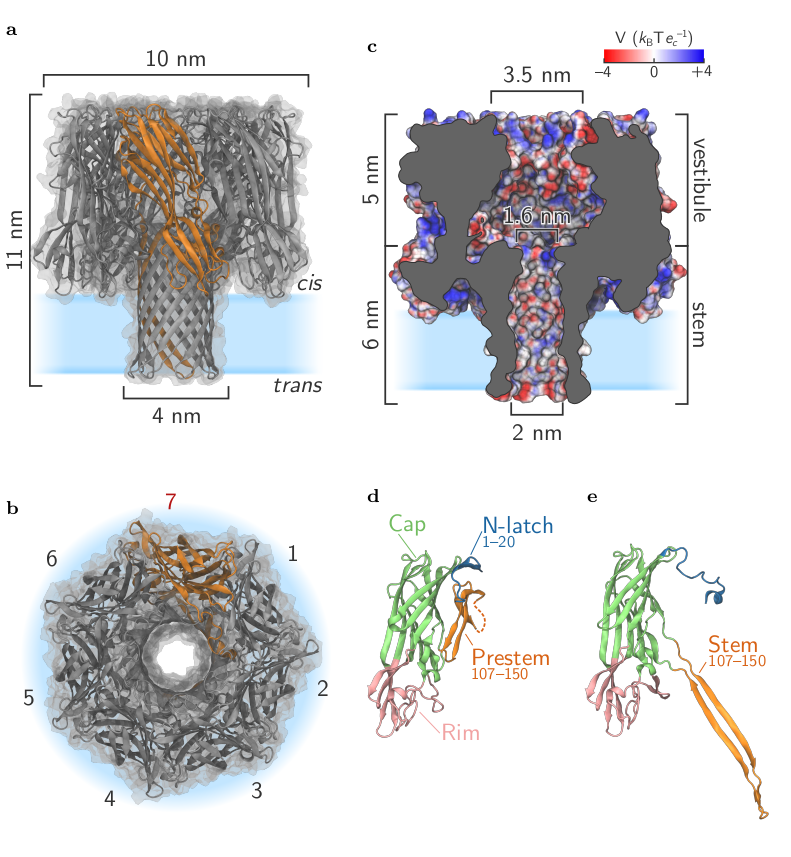
\includegraphics[width=0.5\linewidth]{Figures/alpha-hemolysin.png}
  \caption{write caption}
  \label{adsf}
\end{figure}


\subsection{Cytolysin A (ClyA)}

The Cytolysin A (ClyA) is a larger type of pore forming protein, first found to be
secreted by E. coli strains. The larger size of its lumen allows for different types of
applications, compared to smaller complexes like $\alpha$-HL. Most relevant for this
thesis, is the fact that the larger diameter of the pore's stem allows for translocation
of double stranded DNA.\\

The ClyA pore (PDBID:6MRT[cite]) is an oligomeric complex most typically found in a
 dodecameric configuration is, meaning that there are twelve protomers found in the
complex. In nature there are found small variations on this configuration. The secondary
structure elements consist principally of $\alpha$-helices, making it a member of the $
\alpha$-pore-forming toxins. The protein formation is induced by the hydrophobic
interactions between the $\beta$-hairpin and the solvent. The main structural
rearrangement in this process consists of swinging
out this $\beta$-tongue and inserting it into the membrane. After this transition, the
membrane-bounded monomers oligomerize to from the final pore structure.

Structurally the shape of ClyA resembles that of two hollow cylinders stacked on top of
each other. This cylinder approximation will be important later on in this thesis, where
it will be used to create a simplified model of the nanopore. The total hight of the
complex is
14nm and the maximum width is measured to be 11nm. The lumen's size of this nanopore
differentiates it from the previously discussed $\alpha$-HL. The cis entrance of the
lumen measures 6nm, while the constricted side of the pore is still 3.6nm in diameter. In
contrary to the $\alpha$-HL, the inside surface of ClyA has a net negative charge,
making it cation sensitive. This excess charge will induce an important
 coulomb interaction between the pore and negatively charged analytes.


\begin{figure}[h!]
  \centering
  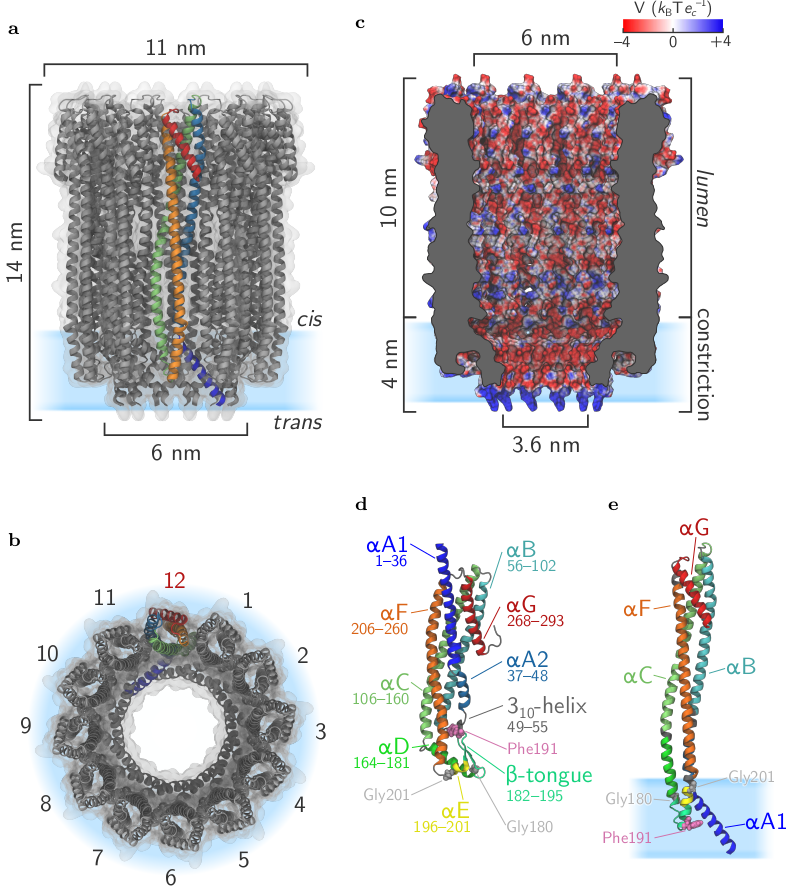
\includegraphics[width=0.5\linewidth]{Figures/cytolysinA.png}
  \caption{write caption}
  \label{adassf}
\end{figure}

\subsection{Ionic current spectroscopy}
In recent years the study of nanopores became a popular research domain, mainly
due to the development of the nanopore-based ionic current spectroscopy. For the case of
biological nanopores, this method depicted in figure ... A lipid bilayer is perforated
using a pore forming protein, for example $\alpha$-HL. The membrane separates two
chambers of a basin filled with a saline solution. When a potential difference is created
over the membrane, the nanopore mediates an ion current between the two sides of the
basin.

This ion current through the pore can accurately be measured. If the pore is empty we
refer to the measured current as the open pore current.  However the applied electric
field also induces forces upon analytes dissolved in the basin. The net result of these
interactions is a flux of analytes towards and in some cases through the nanopore.
Analytes located inside of the nanopore partially block the ion current through the pore,
reducing the measured current. Using machine learning algorithms, the time series of
these current fluctuation can be measured and identified with particular analytes in the
basin. These methods are so precise, that they allow for single cell spectroscopy.

It should be noted that besides these biological nanopores, there are also inorganic
nanopores under development. An example of inorganic nanopres are solid state nanopores,
created by making perforations in a semi-conductor wafer. While currently not as
accessible as biological nanopres, mainly due to their high production cost, this method
has some major advantages. First of all the material properties provide a chemical
robustness not
present in biological nanopores. The production process also allows for easy scalability
and customisability. While currently not as widely used as biological nanopores, due
to their customisability and robustness, solid state nanopores will prove to be an
important asset in future nanotechnology.

\section{Deoxyribonucleic acid (DNA)}

\begin{wrapfigure}{r}{0.23\textwidth}
  \begin{center}
    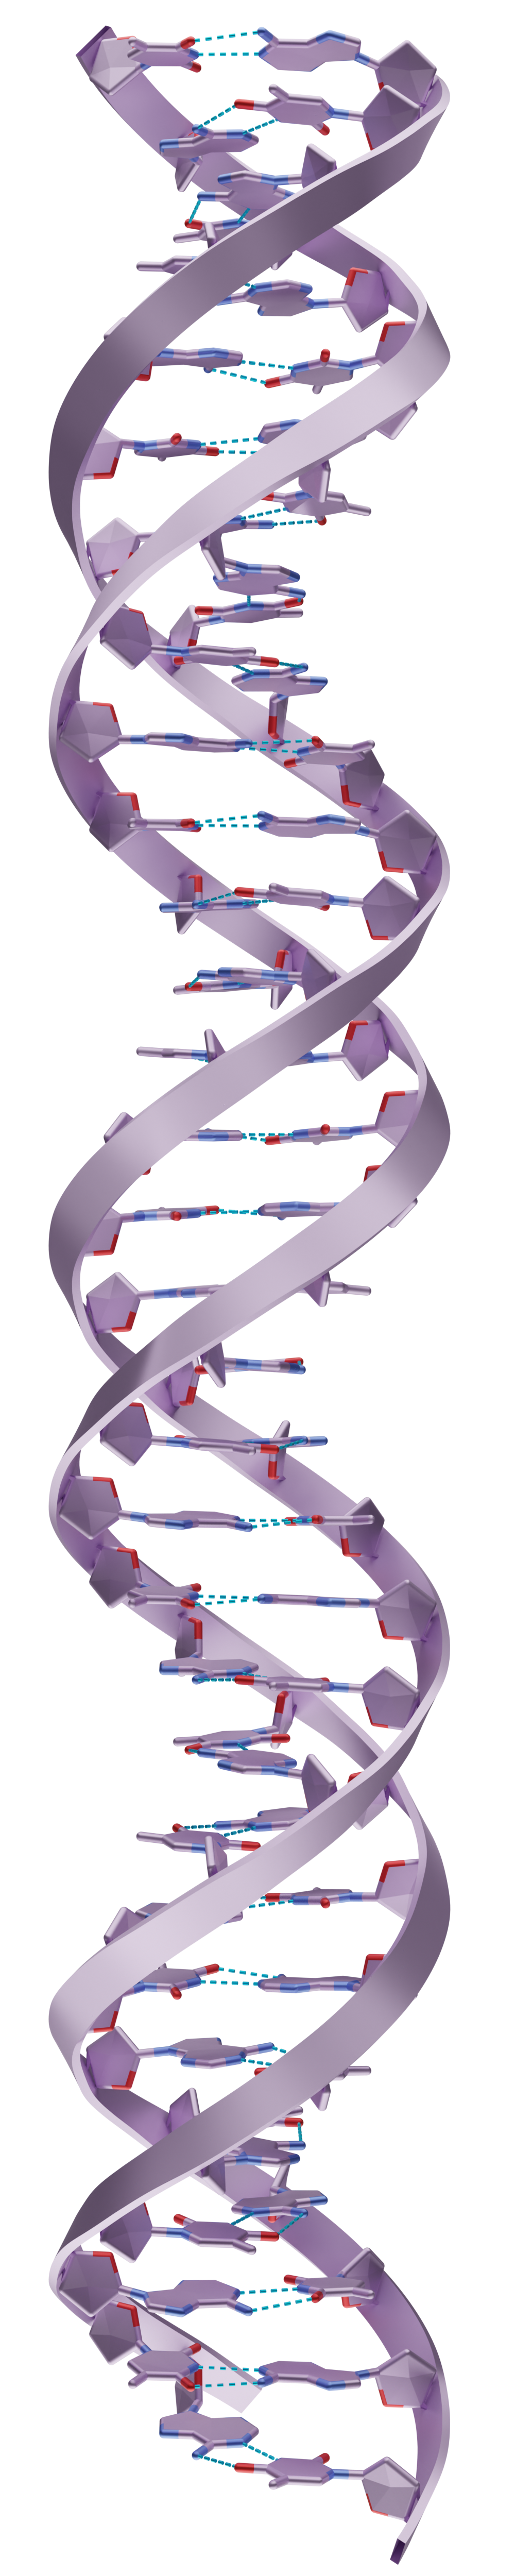
\includegraphics[width=0.20\textwidth]{Figures/cartoon2.png}
  \end{center}
  \caption{caption nog maken}
\end{wrapfigure}

Deoxyribonucleic acid (DNA) is a long biopolymer composed of two strands, commonly found
in its characteristic double helix structure. DNA is most famously know for storing the
genetic code of organisms in the nucleus of their cells. The existence of this genetic
code was already
postulated by the Greek philosopher Aristotle. He developed a heredity theory, based
upon "blueprints", in which he tried to explain why physical traits where passed on from
generation to generation. This theory would go unnoticed until in 1869
Friedrich Meicher discovered a new microscopic substance found on discarded
surgical bandages. He would call this substance "Nuclein" since it originated
form the nucleus of the cell. Later it was found that this new substance, currently known
as "Deoxyribonucleic acid" or DNA, plays an important role as a blueprint for the
perpatuation of living matter.

The structure of DNA was first determined by Rosalind Franklin using X-ray
crystallography. Later this research was published by Watson and Crick [.], who concluded
that DNA consists of two individual strands, coiled around each other in a double helical
structure. Each strand is a chain of monomers, which we call nucleotides. A nucleotide is
made up of a
deoxyribose sugar, phosphate group and one of four nitrogenous bases: cytosine(C),
guanine(G), adenine(A) or thymine(T). The covalent bonds that give both strands structure
are formed between consecutive phosphate groups, which together make up the DNA backbone.
To form the double helix, two backbones are held together by
selective hydrogen bonds occurring between corresponding bases of opposing strands. These
dipole interactions give rise to a selection rule, forming only A-T and C-G base pairs.

Since the binding of the two strands is mediated by hydrogen bonding, association and
dissociation is possible. The study of these processes is called DNA thermodynamics. The
dissociation process of double stranded DNA (dsDNA) is called DNA melting, resulting in
two individual strands of single stranded DNA (ssDNA). The reverse process is called DNA
hybridisation, which is the selective binding of complementary nucleotides to form dsDNA.

The double helix structure of DNA comes in three different types, B-DNA, A-DNA and Z-DNA,
all having a slightly different geometric arrangement. In nature the B-form is most
commonly observed, which is characterised by a right-handed helix and the coplanarity
between the complementary bases as shown in Fig. ... . A helical twist of B-DNA consists
of around 10 base pairs, having a net helical pitch of $0.34 nm$. During this thesis,
when analysing DNA we refer to the B-DNA form.

When studying DNA the statistical theory of polymer physics is a useful tool. An
atomistic resolution is not always needed to accurately describe processes involving
relatively long DNA strands.  Reducing the complexity of DNA to the monomer level is
often justified, allowing us to use more general results in polymer physics.



\section{Polymer Physics}
A polymer is a biomolecule made up of building blocks called monomers, linked together to
from a chain. The configuration of this chain is determined by the position vector of
each monomer, denoted as $\{\boldsymbol{r}_0, \boldsymbol{r}_1, \dots,
\boldsymbol{r}_N\}$.  The link between each consecutive pair of monomers is called the
bond-vector, defined as
$\boldsymbol{u}_i = \boldsymbol{r}_i - \boldsymbol{r}_{i-1}$. During this discussion we
will assume these bonds to be inextensible, i.e. having a fixed
bond length of $|\boldsymbol{u}_i| = a$.\\


Various different models can be used to describe a polymer. The most simple version is
called
the Freely Jointed Chain (FJC). This model is an example of an ideal flexible polymer, in
which excluded volume interactions or polymer bending rigidity are not taken into
account.  In this
model, it is assumed that each bond-vector is completely uncorrelated with its adjacent
bonds. Mathematically this is represented by assigning the bond-vector orientation
an uniform probability distribution
\begin{equation}
    g(\boldsymbol{u}) = \frac{1}{4 \pi a}
    \delta(|\boldsymbol{u}| - a), \\
\end{equation}
where $a$ is the fixed bond length.


The above described model provides a relatively accurate description of long polymers.
However, the assumption that consecutive monomers are uncorrelated becomes
problematic at small length scales. The Kratky-Porod model, or discrete wormlike chain,
solves this problem by taking the energetic cost of bending the polymer into
account. Mathematically this is done introducing a bending rigidity between neighbouring
bonds in the form of a coupling constant, $\kappa >0$. Each polymer configuration is
assigned an energy using the equation,
\begin{equation}
    E_{WLC}= -\kappa \sum_{i=1}^{N} \boldsymbol{\hat{u}_i} \cdot
    \boldsymbol{\hat{u}}_{i+1}
    = -\kappa
    \sum_{i=1}^{N} \cos\theta_i,
    \label{wlc}
\end{equation}
where $\boldsymbol{\hat{u}} = \boldsymbol{u}/a$ is the unit bond-vector and $\theta_i$ is
the angle between neighbouring bond-vectors $\boldsymbol{\hat{u}_i}$ and
$\boldsymbol{\hat{u}_{i+1}}$. The lowest energy state of this discrete wormlike chain is
a straight rodlike configuration, where the bond angles $\theta_i$ are minimized.

To calculate the bond-vector correlation function,  we first determine the partition
function, $Z_{WLC}$, of the system. Identifying the single monomer contributions, this
quantity factorises into a product of single bond-vector partition functions as
\begin{equation}
    \begin{aligned}
        \label{210}
        Z_{\mathrm{WLC}}(N, T)
        &= \int_{0}^{\pi}\dots \int_{0}^{\pi} d \theta_1 \dots d \theta_N \sin \theta_1 \dots
        \sin \theta_N\ e^{\beta \kappa \sum_{i=1}^{N-1} \cos\theta_i}\\
        &= \left[\int_{0}^{\pi} d \theta \sin \theta e^{\beta \kappa \cos
        \theta}\right]^{N}\\
        &= \left[Z_{\mathrm{WLC}}(1, T)\right]^{N},
    \end{aligned}
\end{equation}
where $\beta=1/\kappa_b T$ is the inverse temperature. It rests us to determine the
single bond-vector partition function. Carrying out the integration yields the result,
\begin{equation}
    Z_{\mathrm{WLC}}(1, T)=\int_{0}^{\pi} d \theta e^{\beta \kappa \theta}=\frac{2
    \sinh(\beta \kappa)}{\beta \kappa}.
\end{equation}

%\begin{equation}
%    \left\langle\cos \theta_{i+1}\right\rangle
%    =\frac{\partial \log Z_{\mathrm{WLC}}(1, T)}{\beta \partial \kappa}.
%\end{equation}

From the found partition function we can now determine the bond-vector correlation
function. Using the definition of the partition function, we determine the average cosine
of the angle between consecutive bonds to be,
\begin{equation}
    \begin{aligned}
    \left\langle\cos \theta_{i+1}\right\rangle
    &=\frac{\partial \log Z_{\mathrm{WLC}}(1, T)}{\partial(\beta \kappa)}\\
    &= \frac{1}{\tanh(\beta \kappa)} - \frac{1}{\beta \kappa}.
    \end{aligned}
\end{equation}

Studying the conformation of polymers is often times done assuming a low
temperature or large bending rigidity, where we find
that the above expression simplifies. In the limit, $\beta \kappa \gg 1$, the lowest
order approximation yields,
\begin{equation}
    \langle\cos \theta\rangle \approx 1-\frac{1}{\beta \kappa}.
\end{equation}

Decomposing the bond-vector $\boldsymbol{\hat{u}}_{n+1}$ in terms of an orthonormal
basis, defined by the normal and tangential directions of the preceding vector
$\boldsymbol{\hat{u}}_{n+1}$, gives
\begin{equation}
\boldsymbol{\hat{u}}_{n+1} = \boldsymbol{\hat{u}}_{n} \cos \theta_{n} +
\boldsymbol{\hat{u}}_{n}^{\perp} \sin \theta_{n}.
\end{equation}
This decomposition allows us to express the correlation between distant bond-vectors in
terms of the correlation between neighbouring bonds-vectors. The factorisation
yields
\begin{equation}
\begin{aligned}
    \left\langle\boldsymbol{\hat{u}}_{i} \cdot \boldsymbol{\hat{u}}_{i+m}\right\rangle
    &=\left\langle\boldsymbol{\hat{u}}_{i} \cdot
        \boldsymbol{\hat{u}}_{i+m-1}\right\rangle\left\langle\cos
    \theta\right\rangle = \dots =\langle\cos \theta\rangle^{m},
    % &=\exp \bigg{[} -\frac{n a}{l_{b}} \bigg{]},
\end{aligned}
\end{equation}
where we used the fact that the sinusoidal terms vanish due to symmetry.
Exploring this result in the limit, $\beta \kappa \gg 1$, we find the expression
\begin{equation}
    \left\langle\boldsymbol{\hat{u}}_{i} \cdot \boldsymbol{\hat{u}}_{i+m}\right\rangle =
    e^{m \log(1 - \frac{1}{\beta \kappa})} \approx e^{-na/l_p},
\end{equation}
introducing a new polymer quantity, the bending persistence length

\begin{equation}
    l_b \equiv \frac{a \kappa}{k_{b} T}.
\end{equation}
This general result in polymer physics states that the correlations between bond-vectors
is exponentially decreasing. The defined quantity represents the characteristic
length scale of the polymer, over which the correlations between
bond-vectors is lost.

Two limiting cases can be explored. Firstly, in the
case where the persistence length is much larger then the polymer's length, $l_p \gg na$,
all bond-vectors are correlated, i.e. the polymer approximates a straight rod. For the
reverse case, where $l_p \ll na$, it can easily be shown that the polymer behaves as a
stochastic walk.

The persistence length is a central result in the theory of polymer physics, providing a
measurable quantity related to the bending rigidity of a polymer. During the
simulations performed in this thesis, the notion of bending persistence length is used to
discuss the flexibility of the DNA polymer.


%The end-to-end vector $\boldsymbol{R}$ in the continuum limit. For example can be
%rewritten using the arc-length parameter $s$ where $0 \leq s \leq L$ and $L = Na$ as:
%\begin{equation}
%    \label{hoi}
%    \langle\widehat{u}(q) \cdot \widehat{u}(q+s)\rangle= e^{-s / l_{\mathrm{p}}}.
%\end{equation}
%The continuum version of the end-to-end vector
%\begin{equation}
%    \boldsymbol{R}=\int_{0}^{L} \widehat{u}(s) d s.
%\end{equation}

%\begin{equation}
%\begin{aligned}
%    \left\langle\boldsymbol{R}^{2}\right\rangle
%    &= \int_{0}^{L} d s d s^{\prime}\left\langle\widehat{u}(s) \cdot
%  \widehat{t}\left(s^{\prime}\right)\right\rangle \\
%    &= 2 l_{\mathrm{b}} L\left\{1-\frac{l_{\mathrm{b}}}{L}\left(1-e^{-L /
%l_{\mathrm{b}}}\right)\right\}.
%\end{aligned}
%\end{equation}


\newpage
\section{Computer Simulations}

The theory of classical mechanics is often regarded as the first major breakthrough in
the field of physics. For every aspiring physicist this is still the starting point of
their studies. Unfortunately, getting to know these relatively simple laws of nature,
leads to the inescapable realisation that these theories are expressed in mathematical
formalisms that are only analytically solvable in few idealised scenarios. Applying these
formulas to a problem consisting of just more then two particles already leads to
practically unsolvable equations.\\

Although it is often times not possible to find an exact solution to equations
related to complex physical systems, finding reasonable approximations to their solution
is achievable. One popular method to analyse the dynamics of complex systems is the use
of simulations.\\

\begin{wrapfigure}{r}{0.5\textwidth}
  \begin{center}
    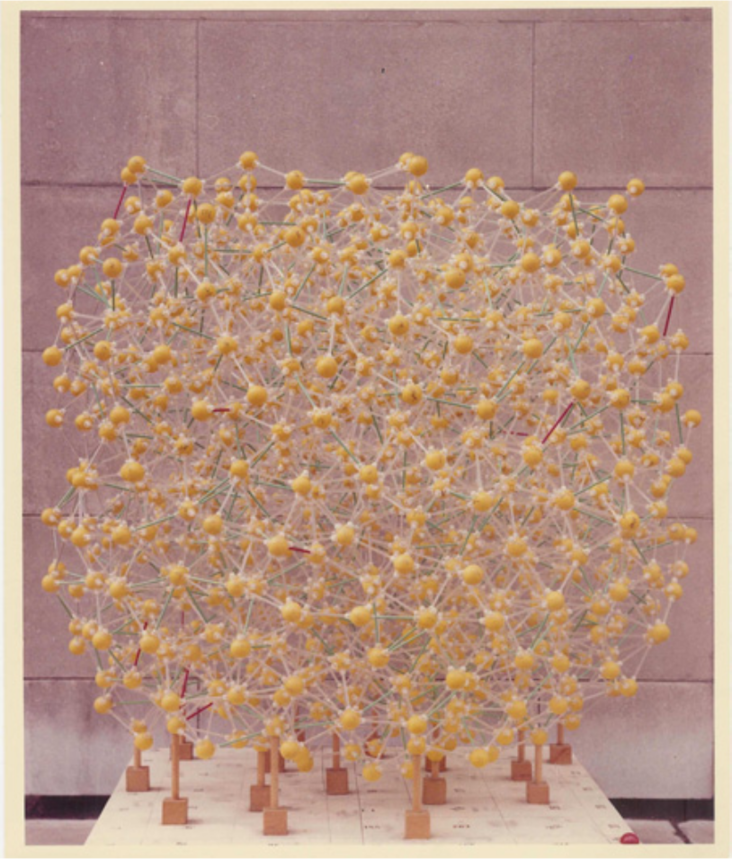
\includegraphics[width=0.38\textwidth]{Figures/WaterModel.png}
  \end{center}
  \caption{Example of an expanded model of a simple liquid (J L Finney, Ph.D thesis)}
\end{wrapfigure}

Simulations have a rich history within physics and engineering, starting even before the
invention of the computer.

\todo{dit weg laten??? misschien te veel bla bla}
An example of one of these mechanical simulations is the Waterloopkundig Laboratorium or
currently the waterloopbos, a scale model of important
Dutch waterways, where the influence of waves on harbours and docks was studied. This
simulation provided revolutionary insights into the behaviour of water and played an
important part in the design of the famous Delta Works.\\

Another more relevant example is the use of mechanical simulations to study the
structure of water.  In the early 20th century physicist J.D. Bernal and his fellow
researchers build various ball and stick models of water to analyse the possible 3D
configurations of water molecules in a liquid. Their research eventually explained the
peculiar physical properties of water from a atomistic perspective. However useful these
mechanical simulations turned out to be, the biggest drawback of the method was the
extreme cost of labour involved with their construct. As Bernal alluded to in his
famous 1962 lecture,

\begin{quote}
\dots I took a number of rubber balls and stuck them together with rods of a
selection of different lengths ranging from 2.75 to 4 inch. I tried to do this in the
first place as casually as possible, working in my own office being interrupted every
five minutes or so and not remembering what I had done before the interruption.\dots
\end{quote}

After the first computer simulations where performed in the Los Alamos labs, the
popularity of simulations rapidly increased. The remarkable explanatory power of
simulations, combined with the relative easy construction of computer models, lead to a
fast adoption of computer simulations in the scientific community. Within the context of
this thesis, computer simulations are used to study the mechanics of
the DNA polymer. Due to the high number of atoms in a typical system, it is generally
not possible to find an analytical solution to their equations of motion. In this
context, simulations are often used to gain an insight into the complex dynamics of the
system and guide the developments of more simple approximate theories. The simulations
act as a bridge between the microscopic constituents of the systems and the macroscopic
properties we want to understand.


\subsection{Molecular Dynamics Simulations}
Molecular Dynamics (MD) is a computer simulation technique, used to analyse
the dynamics of a classical many-body system. The central idea of this method is to
generate all the trajectories in a system of $N$ particles by numerically
integrating the classical equations of motion,
\[
m_i \frac{d^2 \boldsymbol{r_i}}{dt^2} = \boldsymbol{f_i}, \quad \boldsymbol{f_i} = -
    \frac{\partial}{\partial \boldsymbol{r_i}} \mathcal{U}_i, \quad for\ i \in N.
\]
The motion of the particles are governed by the forces $f_i$ acting upon them, which are
usually derived from the interaction potentials $U_i$.
Solving these differential equations is achieved by employing a discretized time
integration scheme.  Algorithm 1 shows the typical structure of a molecular dynamics
simulation. The discretization resolution is conventionally called the time step of the
simulations denoted by $\Delta t$.\\

\noindent There are a large number of different integrations schemes that one can choose
from, where the choice depends entirely on the system at hand.
When working with an isolated system -- i.e. microcanonical ensemble --, logically an
energy conserving integrator is needed. The canonical
choice for this type of integration scheme is the Velocity-Verlet algorithm. This
algorithm is an example of leapfrog integration, where the updating of the positions
and velocities are interleaved at different points in time. The major strength of this
type of algorithm is that it turns out to be a symplectic integrator, which means the
errors on the conserved energy are bounded.

On the other hand, when a system is in contact with a thermal reservoir --i.e. canonical
ensemble-- not the total energy is conserved, but rather the temperature of the
simulation is fixed. To achieve this, a thermostat is implemented in the MD
simulation. A typical thermostat attempts to negate any drift in temperature by
appropriately importing or exporting energy to the system after each timestep.
Poplular examples of thermostats are the Nos\'e-Hoover thermostat or the Langevin
thermostat.  The latter regulates the temperature by introducing an implicit solvent to
the simulation that gives rise to random thermal kicks. The resulting equations of motion
are the Langevin equations given by,

\begin{equation}
    m_i \frac{d^2 \boldsymbol{r}_i}{dt^2} = - \nabla \mathcal{U}_i - \gamma_i \frac{d
    \boldsymbol{r}_i}{d t} +
    \xi_i(t),
\end{equation}
where $\gamma_i$ is known  as the friction coefficient and $\xi_i(t)$ a random force
acting upon the particles. The combination of the last two terms fully capture the
statistical consequences of the solvent interacting with the system.


\begin{algorithm}
    \SetKwFunction{isOddNumber}{isOddNumber}
    \SetKwInOut{KwIn}{Input}

    \KwIn{Configuration of the system at $t=0$}

    $newList = [\ ]$

    \tcc{For odd elements in the list, we add 1, and for even elements, we add 2.}

    \For{$i \leftarrow 0$ \KwTo $n-1$}{
        \eIf{$\isOddNumber(a_i)$}{

            $newList.append(a_i + 1)$ \tcp*[f]{Some thought-provoking comment.}
         }{
            \tcp{Another comment}
            $newList.append(a_i + 2)$
         }
    }

    \KwRet{$newList$}
    \caption{The Velocity Verlet algorithm}
\end{algorithm}

% \begin{center}
% 	\begin{tikzpicture}[
% 	squarednode/.style={rectangle, draw=blue!60, fill=blue!5, very thick, minimum width=50mm,
% 	minimum height=5mm},]
% 	%Nodes
% 	\node[squarednode]      (step1)                        {1};
% 	\node[squarednode]      (step2)       [below= 3mm of step1] {2};
% 	\node[squarednode]      (step3)       [below= 3mm of step2] {3};
% 	\node[squarednode]      (step4)       [below= 3mm of step3] {4};
% 	\node[squarednode]      (step5)       [below= 3mm of step4] {5};
% 	\node[squarednode]      (step6)       [below= 3mm of step5] {6};
% 	\node[squarednode]      (step7)       [below= 3mm of step6] {7};
% 	\node[squarednode]      (step8)       [below= 3mm of step7] {8};
%
% 	%Lines
%     \draw[very thick, ->] (step1.south) -- (step2.north);
% 	\draw[very thick, ->] (step2.south) -- (step3.north);
% 	\draw[very thick, ->] (step3.south) -- (step4.north);
% 	\draw[very thick, ->] (step4.south) -- (step5.north);
%     \draw[very thick, ->] (step5.south) -- (step6.north);
% 	\draw[very thick, ->] (step6.south) -- (step7.north);
% 	\draw[very thick, ->] (step7.south) -- (step8.north);
% 	\draw[very thick, ->] (step8.west)  -- +(-0.4,0) |-(step2.west);
% 	\end{tikzpicture}
% \end{center}

\subsection{Coarse Grained modelling}
As most thing do, molecular dynamics simulations have their pitfalls. A commonly
encountered problem is the rapidly increasing computational cost, when the number of
particles in the system increase. If not addressed, this would limit the scope of MD
simulations to systems of a few particles over short time-scales.\\

During these simulations the most costly calculations involve the non-bonded
interactions in the system. These interatomic interactions make the computational
complexity for rudimentary MD simulations scale as $O(N^2t)$, where $N$ is the number of
particles in the system and $t$ the simulation time. This bad scaling behaviour comes
from the fact, that for each individual particle all the other particles are contributing
to its interaction potential. To improve this scaling behaviour, the non-bonded
interactions in a MD simulation are almost always truncated. This localization of the
interatomic interactions has the nice effect that not all atoms are involved in every
calculation. Efficient algorithms, like the multigrid method, have been derived to
improve the scaling complexity of MD simulations up to $O(Nt)$.\\

Coarse graining is a method to further optimize molecular dynamics simulations.
In contrary to all atom simulations, where each atom is explicitly represented in the
simulation, in coarse grained simulations multiple atoms are grouped together to form
generalised pseudo-atoms with their respective pseudo-interaction.

There are two distinctly different ways to construct a coarse grained model. The first
method starts from the all atom model of the system and generalises nearby atoms into
larger pseudo-atoms, this is called the bottom up approach. The second method focuses
more on the precise reproduction of a system's thermodynamical properties, rather than
the precise small scale dynamics. Here larger pseudo-atoms are designed, based upon
repeating structures in the system, after which the pseudo-interactions are tweaked to
accurately reproduce the system's dynamics.

In the case of DNA simulations, coarse graining turned out to be a very important method.
Previous all atom simulations of DNA polymers were restricted to simulations of less then
hundred baisepairs over only a few microseconds. Studying large scale systems, often
encountered in DNA technology, was only possible after the development of coarse grained
models. A few examples of commonly used coarse grained models of DNA are Martini, 3SPN
and oxDNA.

\begin{figure}[htpb]
    \centering
    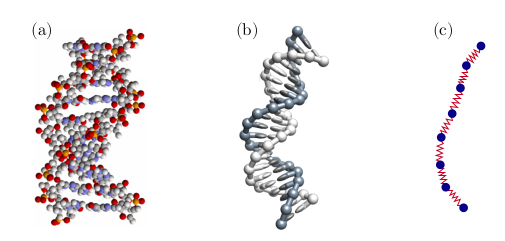
\includegraphics[width=0.6\linewidth]{Figures/CoarseGrained.png}
    \caption{zelf nog namaken met blender!!!}%
    \label{fig:Figures/CoarseGrained}
\end{figure}


\cleardoublepage

\chapter{The DNA Nanopiston}
\vspace{-1cm}
\epigraph{Given for one instant an intelligence which could comprehend all
the forces by which nature is animated and the respective positions
of the beings which compose it, if moreover this intelligence were vast
enough to submit these data to analysis, it would embrace in the same
formula both the movements of the largest bodies in the universe and
those of the lightest atom; to it nothing would be uncertain, and the
future as the past would be present to its eyes.}
{--- \textup{Pierre-Simon Laplace}}

\chapter{Adapting the Model}
\vspace{-1cm}
\epigraph{All models are wrong, but some are useful.}
{--- \textup{George Box}}
\section{OxDNA}

\begin{wrapfigure}{r}{0.45\textwidth}
  \begin{center}
    \includegraphics[width=0.42\textwidth]{Figures/oxDNA_model.png}
  \end{center}
  \caption{Structure of the OxDNA model with the different interactions.
          Figure was taken form [].}
\end{wrapfigure}

OxDNA is a coarse-grained model of DNA developed by Thomas E. Ouldridge et al. at Oxford
university. The central aim of the project was to develop a coarse-grained model of DNA
that could be used in the design of DNA technology. For the development of these
technologies a model was needed that accurately captured the structural, mechanical and
thermodynamical properties of DNA while keeping the computational cost low.

The OxDNA model represents each nucleotide in the DNA strand as a rigid unit. Each rigid
nucleotide has three independent interaction sites, each capturing a different aspect of
the model. The interactions between these pseudo atoms are next compared to experimental
data to tweak the interactions, characterising the approach as "top down"
coarse-graining. The interactions defined in the OxDNA model can be summarized as,

\begin{equation}
  \begin{aligned}
    V = \sum_{\text{nearest neighbours}} \bigg[ V_{\text{backbone}} + V_{\text{stack}} +
    V^{'}_{\text{exc}}\bigg]\\
    + \sum_{\text{other pairs}} \bigg[V_{\text{HB}} + V_{\text{cross stacking}} +
    V_{\text{exc}} + V_{\text{coax stack}}\bigg].
  \end{aligned}
\end{equation}

The first interaction site is the hydrogen-bonding/base excluded volume site,
incorporating the hybridisation of complementary nucleotides into the model. The
hydrogen-bonding interactions are not fixed, allowing for OxDNA to simulate dsDNA, ssDNA
and their thermodynamic transitions.

The second interaction site is an excluded volume interaction located at the backbone.
These interactions simulate the covalent bonding between consecutive phosphate groups
using the FENE (finitely extensible nonlinear elastic) bond type.

The last interaction site is again located at base where it provides a base stacking
interaction between consecutive nucleotides. The nucleotides stacking in DNA is crucial
for the formation of the characteristic helical structure. Using these stacking
interactions this structure is implicitly imposed in the model. Contrasting the common
approach of explicitly imposing the Double helix structure in other coarse grained-models
like 3SPN and Martini. This implicit structure allows for the unstacking of nucleotides,
which especially in ssDNA is an important contribution to the flexibility of the strand.

During the simulations of the DNA Nanopiston both the flexibility of the single stranded
DNA strands and the hybridisation reactions play an important role. Since both of these
aspect of DNA are accurately captured by the OxDNA model, it provides a logical choice
for our simulations. The low number of degrees of freedom in the model, allows us to
simulate computationally intensive simulations like DNA hybridisation.


% APPENDIX
\begin{appendices}
\addtocontents{toc}{\protect\setcounter{tocdepth}{1}}
\chapter{One Dimensional Confined Diffusion}

This appendix provides a detailed description of the motion of a Brownian particle
confined to a one dimensional domain. Due to the stochastic nature of this motion, we
will discuss the evolution of the probability density function $\phi(x,t)$, which
represents the probability of finding the particle on the position $x$ at time t.
Once the evolution of this probability function is known, the statistical properties can
be evaluated. Here, we will discuss the Mean Square Displacement (MSD), as it is used to
analyse the motion of the $0nt$ mixed rotaxane.\\
A central result in statistical mechanics is that the evolution of
$\phi$ is  described by the diffusion equation, given by
\begin{equation}
  \frac{\partial \psi}{\partial t} =  D \frac{\partial^2 \psi}{\partial x^2}, \quad
  \label{eq:diff}
\end{equation}
where D is the diffusion coefficient of our particle.
The confinement is imposed through reflecting boundary conditions at $x=0$ and $x=L$,
which is equivalent to imposing a
vanishing particle current at the boundaries of our domain, $j = - D \frac{\partial
\psi}{\partial x} = 0$. Solving equation \ref{eq:diff} can be done using the
method of
separation of variables, where we assume that the solution can be expressed as $
\psi(x,t) = f(x)g(t)$. Upon this substitution Eq. \ref{eq:diff} becomes,
\begin{equation}
  \frac{\dot{g}}{g} = \frac{\ddot{f}}{f} = - \alpha,
\end{equation}
where the two expressions are implied to be constant since the variables are independent.
The partial differential equation is now treated as two seperate ordinary differential
equations, for which we find,

\begin{align}
t:\quad \dot{g} = - \alpha g(t) \Rightarrow g(t) = e^{-\alpha t},
\end{align}

\begin{align}
  x:\quad D \ddot{f} = - \alpha f(x) \Rightarrow f(x) &= A \sin(K x) + B \cos(Kx)\\
  &= B \cos(\frac{\pi n x}{L}).
\end{align}
In the latter expression the boundary conditions impose that $A=0$ and constrain the
parameters by the relation,
\begin{align}
  \frac{\alpha}{D} = \frac{\pi^2 n^2}{L^2}.
\end{align}
By substituting the found results into the assumed form of the solution, we find the
general solution to the confined diffusion equation as the linear combination,
\begin{align}
  \psi(x,t) &= \sum_{n=0}^{+\infty} C_n \cos\Big(\frac{\pi n x}{L}\Big) e^{- \frac{D\pi^2
  n^2}{L^2}t}.
\end{align}
At time $t=0$ the particle is assumed to be found at $x_0$ resulting in the initial
condition,
\begin{align}
  \psi(x, 0) = \delta(x-x_0) = \sum_{n=0}^{+ \infty} C_n \cos(\frac{\pi n x}{L}).
\end{align}
Imposing this initial condition on the found general solution of the confined diffusion
equation gives,
\begin{align}
  \psi(x, t)=\frac{1}{L} \Bigg[ 1 + \sum_{n=1}^{+\infty} \cos\Big(\frac{\pi n
  x_0}{L}\Big) \cos\Big(\frac{\pi n x}{L}\Big) e^{- \frac{D\pi^2  n^2}{L^2}t}\Bigg].
\end{align}
This expression describes the behaviour of a Brownian particle in a one dimensional
confined domain. Using the found expression the MSD is calculated to be,
\begin{align}
  \langle \Delta x^2 \rangle &= \langle(x-x_0)^2\rangle\\&= \frac{L^2}{6}\Bigg[1 -
  \frac{96}{\pi^4}
  \sum_{k=0}^{+\infty} \frac{1}{(2k+1)^4} e^{- \frac{D(2k+1)^2 \pi^2}{L^2}t}\Bigg].
\end{align}
As expected, the mean square distances saturates to $\langle \Delta x^2 \rangle = L^2/6$
in the long-time limit $t \gg L^2 / D.$ To explore the other limiting case $t \ll L^2/D
$, we perform a Taylor expansion of the exponential and find,
\begin{align}
  \langle \Delta x^2 \rangle &= \frac{L^2}{6} - \frac{16 L^2}{\pi^4} \sum_{k=0}^{\infty}
  \frac{1}{(2k+1)^4} + \frac{16 D t}{\pi^2} \sum_{k=0}^{\infty} \frac{1}{(2k+1)^2} +
  \mathcal{O}\bigg(\frac{D^2 t^2}{L^4}\bigg).
\end{align}
Using the two convergent series,
\begin{equation}
  \sum_{k=0}^{\infty} \frac{1}{(2k+1)^2} = \frac{\pi^2}{8} \qquad \text{and} \qquad
  \sum_{k=0}^{\infty} \frac{1}{(2k+1)^4} = \frac{\pi^4}{96}
\end{equation}
the free diffusion is recovered at short time scales,\cite{BICKEL200724}
\begin{equation}
  \langle \Delta x^2 \rangle = 2Dt \qquad \text{for }\,\, t \ll L^2/D.
\end{equation}

\end{appendices}

% BIBLIOGRAPHY
%\addcontentsline{toc}{chapter}{Bibliography}
\bibliographystyle{apalike}
\begin{multicols}{2}
\begin{smallfont}
\bibliography{Bibliography/thesis.bib}
\end{smallfont}
\end{multicols}
\cleardoublepage

\chapter*{Acknowledgements}
\addcontentsline{toc}{chapter}{Acknowledgements}
...
 \cleardoublepage


% Back side of book
\cleartoleftpage{} % Make sure the back page is at an even page number


% ----------------------- Achterblad ------------------------------
% Vergeet niet de tekst aan te passen:
% - Afdeling
% - Adres van de afdeling
% - Telefoon en faxnummer
% -----------------------------------------------------------------
\thispagestyle{empty}
\sffamily
%
\begin{textblock}{191}(102,-22)
{\color{blueline}\rule{160pt}{5.5pt}}
\end{textblock}
%
\begin{textblock}{191}(157,-22)
{\color{blueline}\rule{5.5pt}{59pt}}
\end{textblock}
%
\begin{textblock}{183}(-35,-22)
\textblockcolour{}
\flushright
\fontsize{7}{7.5}\selectfont
\textbf{DEPARTEMENT NATUURKUNDE EN STERRENKUNDE}\\
Celestijnenlaan 200d bus 2412\\
3000 LEUVEN, BELGI\"{E}\\
tel. + 32 16 32 71 24\\
fys.kuleuven.be\\
\end{textblock}
%
\begin{textblock}{191}(145,-16)
\textblockcolour{}
\includegraphics*[height=16.5truemm]{Figures/sedes}
\end{textblock}
%
\begin{textblock}{191}(-31,224)
{\color{bluetitle}\rule{544pt}{55pt}}
\end{textblock}


\end{document}
